% \documentclass[review]{elsarticle}
\documentclass[utf8, babel, sor, jor, amsmath,amssymb, reprint]{elsarticle} %удалить перед отправкой
\usepackage[T2A]{fontenc} %удалить перед отправкой
\usepackage[utf8x]{inputenc} %удалить перед отправкой
\usepackage[english,russian]{babel} %удалить перед отправкой
\graphicspath{{images/}}

\usepackage{lineno,hyperref}
\usepackage{algorithm}
\usepackage{algorithmic}
\modulolinenumbers[5]

\journal{Journal of \LaTeX\ Templates}

%%%%%%%%%%%%%%%%%%%%%%%
%% Elsevier bibliography styles
%%%%%%%%%%%%%%%%%%%%%%%
%% To change the style, put a % in front of the second line of the current style and
%% remove the % from the second line of the style you would like to use.
%%%%%%%%%%%%%%%%%%%%%%%

%% Numbered
%\bibliographystyle{model1-num-names}

%% Numbered without titles
%\bibliographystyle{model1a-num-names}

%% Harvard
%\bibliographystyle{model2-names.bst}\biboptions{authoryear}

%% Vancouver numbered
%\usepackage{numcompress}\bibliographystyle{model3-num-names}

%% Vancouver name/year
%\usepackage{numcompress}\bibliographystyle{model4-names}\biboptions{authoryear}

%% APA style
%\bibliographystyle{model5-names}\biboptions{authoryear}

%% AMA style
%\usepackage{numcompress}\bibliographystyle{model6-num-names}

%% `Elsevier LaTeX' style
\bibliographystyle{elsarticle-num}
%%%%%%%%%%%%%%%%%%%%%%%


\usepackage{xcolor}
\newcommand{\todo}[1] {\textcolor{red}{#1}} %%for TODO comments
\def\l{\left\langle}
\def\r{\right\rangle}

\usepackage{mathrsfs}
\usepackage{amsmath}
\usepackage{amssymb}%



\begin{document}

\begin{frontmatter}


\title{Ground state search 2D Ising model}

\author[mainaddress, secondaryaddress]{Viacheslav Trukhin\corref{mycorrespondingauthor}}
\ead{trukhin.vo@dvfu.ru}

\author[mainaddress, secondaryaddress]{Konstantin Nefedev\corref{mycorrespondingauthor}}
\ead{nefedev.kv@dvfu.ru}

\author[mainaddress]{Egor Prokhorov\corref{mycorrespondingauthor}}
\ead{prokhorov.ei@dvfu.ru}

\address[mainaddress]{Far Eastern Federal University, Vladivostok, Russky Island, 10 Ajax Bay, 690922, the Russian Federation}
\address[secondaryaddress]{Institute of Applied Mathematics, Far Eastern Branch, Russian Academy of Science, Vladivostok, Radio 7, 690041, the Russian Federation}

\begin{abstract}


\end{abstract}


\begin{keyword}
Ising model, GPU and CPU high performance calculations, spin ice, spin glass, statistical thermodynamics.

\end{keyword}


\end{frontmatter}

\linenumbers
\newpage
\tableofcontents

\newpage
\section{Введение}



\section{Решение исчерпывающим перебором}

Модель спинового стекла Эдвардса-Андерсена представляет собой плоскую решетку Изинга:

\begin{equation}
	E = -\sum J_{ij} S_i S_j
	\label{eq:ising_energy}
\end{equation}

, где обменные интегралы $J$ могут принимать значения +1 или -1 создавая таким образом приближение аморфных материалов

Для решения такой цепочки из трёх спинов статистическая сумма
принимает вид:

\begin{equation}
	Z = e^{3\beta - 3\beta h} + 3e^{\beta - h - \beta} + 3e^{\beta h - \beta} + e^{3\beta + 3\beta h}
	\label{eq:stat_3}
\end{equation}

\section{Решение методом декомпозиции}

Рассматривая разные квадратные решётки из четырёх спинов взаимодействующих лишь с ближайшими соседями, можно заметить, что фрустрация в основном состоянии обязательно появляется, если в системе три обменных интеграла одного знака, а четвёртый другого.

\begin{figure}[h]
	\centering
	\resizebox{120px}{50px}{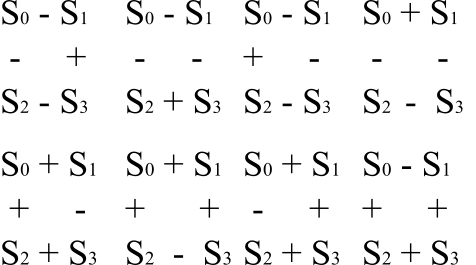
\includegraphics{2x2.1.png}}
	\caption{Фрустрированные квадратные системы}
	\label{fig:label}
\end{figure}

Тогда логично предположить, что если система состоит из двух таких подсистем, то для минимизации энергии фрустрированная пара должна быть расположена на пересечении этих подсистем.
На Рис.2 пример решётки, состоящей из двух квадратных фрустрированных подсистем. Фрустрированной парой спинов будет пара $S_1$,$S_4$.

\begin{figure}[h]
	\centering
	\resizebox{75px}{55px}{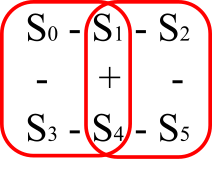
\includegraphics{3x2.png}}
	\caption{Решётка,состоящая из двух квадратных фрустрированных подсистем}
	\label{fig:label}
\end{figure}

Таким образом, зная где расположена фрустрированная пара спинов, а следовательно, и где расположены не фрустрированные пары, можно найти основное состояние системы просто расставляя значение спинов по порядку. Метод полного перебора подтверждает правильность данного решения.

Рассматривая решётки больших размеров (Рис.3), во многих случаях фрустрированные подсистемы будут иметь несколько пар, расположенных на пересечении. В таких случаях подсистемы образуют кластер. В решётке на Рис.3 образуется кластер, в который входят спины $S_1$, $S_2$, $S_3$, $S_4$, $S_{10}$, $S_{11}$, $S_{12}$, $S_{13}$, $S_{21}$, $S_{22}$. В кластере необходимо выбрать фрустрированными пары, находящиеся на пересечении так чтобы такая пара была в подсистеме только одна. Если в каком-то состоянии подсистема осталась без выбранной пары в силу невозможности её расположения на пересечении подсистем, выбирается одна из трёх оставшихся в подсистеме пар, по возможности та, которая не будет возбуждать другие подсистемы, не входящие в кластер .Это можно сделать с помощью полного перебора состояний пар, где состояние пары может принимать только два значения: пара фрустрирована и пара не фрустрирована.

\begin{figure}[h]
	\centering
	\resizebox{310px}{220px}{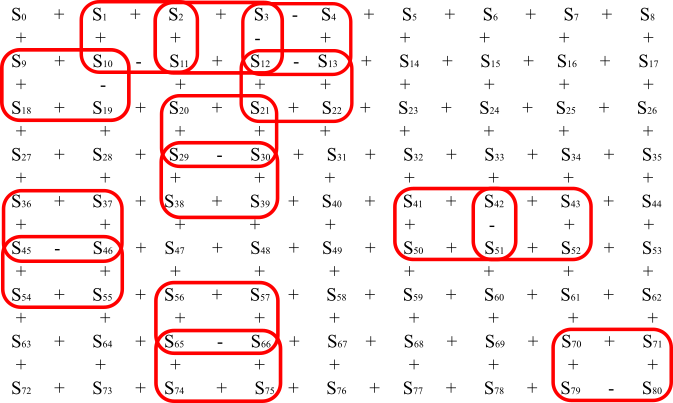
\includegraphics{9x9.png}}
	\caption{Квадратная решётка из 81 спина}
	\label{fig:label}
\end{figure}


\section{Благодарности}

 

\bibliography{mybibfile}


\end{document}